% Important: If latex complains about unicode characters,
% please use "\usepackage[utf8x]{inputenc}" in your preamble
% You can change the size of the picture by putting it into the construct:
% 1) \resizebox{10cm}{!}{"below picture"} to scale horizontally to 10 cm
% 2) \resizebox{!}{15cm}{"below picture"} to scale vertically to 15 cm
% 3) \resizebox{10cm}{15cm}{"below picture"} a combination of above two
% It is not recomended to use the scale option of the tikzpicture environment.
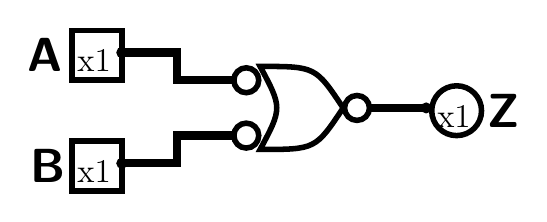
\begin{tikzpicture}[x=1pt,y=-1pt,line cap=rect]
\def\logisimfontA#1{\fontfamily{cmr}{#1}} % Replaced by logisim, original font was "SansSerif"
\def\logisimfontB#1{\fontfamily{Microsoft Sans Serif}{#1}}
\definecolor{custcol_0_0_0}{RGB}{0, 0, 0}
\definecolor{custcol_ff_ff_ff}{RGB}{255, 255, 255}
\draw [line width=3.0pt, custcol_0_0_0 ]  (39.0,15.0) -- (59.0,15.0) -- (59.0,25.0) -- (79.0,25.0) ;
\draw [line width=3.0pt, custcol_0_0_0 ]  (39.0,55.0) -- (59.0,55.0) -- (59.0,45.0) -- (79.0,45.0) ;
\draw [line width=3.0pt, custcol_0_0_0 ]  (129.0,35.0) -- (149.0,35.0) ;
\draw [line width=2.0pt, custcol_0_0_0]  (160.0,36.0) ellipse (9.0 and 9.0 );
\logisimfontA{\fontsize{12pt}{12pt}\selectfont\node[inner sep=0, outer sep=0, custcol_0_0_0, anchor=base west] at  (153.0,42.0)  {x1};}
\logisimfontB{\fontsize{16pt}{16pt}\sffamily\fontseries{bx}\selectfont\node[inner sep=0, outer sep=0, custcol_0_0_0, anchor=base west] at  (171.0,42.0)  {Z};}
\fill [line width=2.0pt, custcol_0_0_0]  (149.0,35.0) ellipse (2.0 and 2.0 );
\draw [line width=2.0pt, custcol_0_0_0]  (84.0,25.0) ellipse (4.5 and 4.5 );
\draw [line width=2.0pt, custcol_0_0_0]  (84.0,45.0) ellipse (4.5 and 4.5 );
\draw [line width=2.0pt, custcol_0_0_0 ]  (119.0,35.0) .. controls  (109.0,20.0)  ..  (89.0,20.0) .. controls  (97.0,35.0)  ..  (89.0,50.0) .. controls  (109.0,50.0)  ..  (119.0,35.0) -- cycle ;
\draw [line width=2.0pt, custcol_0_0_0]  (124.0,35.0) ellipse (4.5 and 4.5 );
\draw [line width=2.0pt, custcol_0_0_0 ]  (21.0,7.0) -- (38.0,7.0) ;
\draw [line width=2.0pt, custcol_0_0_0 ]  (39.0,7.0) -- (39.0,24.0) ;
\draw [line width=2.0pt, custcol_0_0_0 ]  (39.0,25.0) -- (22.0,25.0) ;
\draw [line width=2.0pt, custcol_0_0_0 ]  (21.0,25.0) -- (21.0,8.0) ;
\logisimfontA{\fontsize{12pt}{12pt}\selectfont\node[inner sep=0, outer sep=0, custcol_0_0_0, anchor=base west] at  (23.0,22.0)  {x1};}
\logisimfontB{\fontsize{16pt}{16pt}\sffamily\fontseries{bx}\selectfont\node[inner sep=0, outer sep=0, custcol_0_0_0, anchor=base west] at  (5.0,22.0)  {A};}
\fill [line width=2.0pt, custcol_0_0_0]  (39.0,15.0) ellipse (2.0 and 2.0 );
\draw [line width=2.0pt, custcol_0_0_0 ]  (21.0,47.0) -- (38.0,47.0) ;
\draw [line width=2.0pt, custcol_0_0_0 ]  (39.0,47.0) -- (39.0,64.0) ;
\draw [line width=2.0pt, custcol_0_0_0 ]  (39.0,65.0) -- (22.0,65.0) ;
\draw [line width=2.0pt, custcol_0_0_0 ]  (21.0,65.0) -- (21.0,48.0) ;
\logisimfontA{\fontsize{12pt}{12pt}\selectfont\node[inner sep=0, outer sep=0, custcol_0_0_0, anchor=base west] at  (23.0,62.0)  {x1};}
\logisimfontB{\fontsize{16pt}{16pt}\sffamily\fontseries{bx}\selectfont\node[inner sep=0, outer sep=0, custcol_0_0_0, anchor=base west] at  (6.0,62.0)  {B};}
\fill [line width=2.0pt, custcol_0_0_0]  (39.0,55.0) ellipse (2.0 and 2.0 );
\end{tikzpicture}

